\section{Einleitung}

\begin{frame}
\frametitle{Inhaltsübersicht}
\tableofcontents%[pausesections]
\end{frame}

\begin{frame}[fragile]
  \frametitle{synthetische Polymere}
       \begin{tabular}{cl}
         \begin{tabular}{c}
           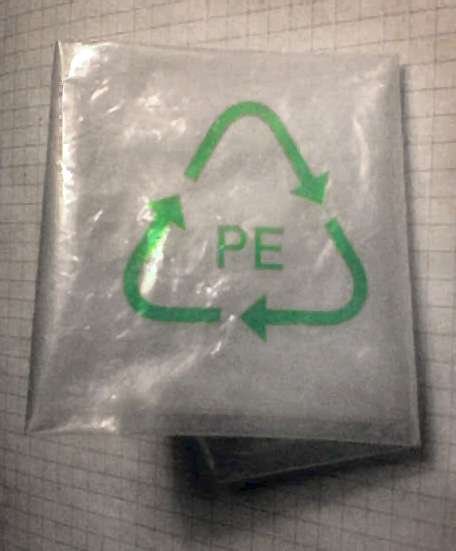
\includegraphics[width=0.2\textwidth]{Plots/Polyethylene.jpg}
           
\includegraphics[width=0.2\textwidth]{Plots/polyethylene-structure.png}\\
           
\includegraphics[width=0.5\textwidth]{Plots/pe03.png}
           \end{tabular}
           & \begin{tabular}{l}
             \parbox{0.5\linewidth}{
             \begin{itemize}
               \item Polyethylen (PE)
               \item Polyvinylchlorid (PVC)
               \item Polystyrol (PS) \\
             \end{itemize}
             \begin{tiny}
                Quellen:\\
                oben links: \\ \url{https://en.wikipedia.org/wiki/Polyethylene##/media/File:Polyethylene.jpg} \\
                oben rechts: \\ \url{https://de.wikipedia.org/wiki/Polyethylen##/media/File:Polyethylene_repeat_unit.svg}\\
                unten: \url{https://www.pslc.ws/macrog/pe.htm}
             \end{tiny}
             }
             \end{tabular}  \\
         \end{tabular}
\end{frame}

\begin{frame}
  \frametitle{biologische Polymere}
	\begin{minipage}{0.3\textwidth}
    \begin{itemize}
      \item dsRNS
      \item F-Aktin
      \item Mikrotubuli
    \end{itemize} %\vspace{2.5cm}\\
	\end{minipage}
	\hfill
	\begin{minipage}{0.3\textwidth}
	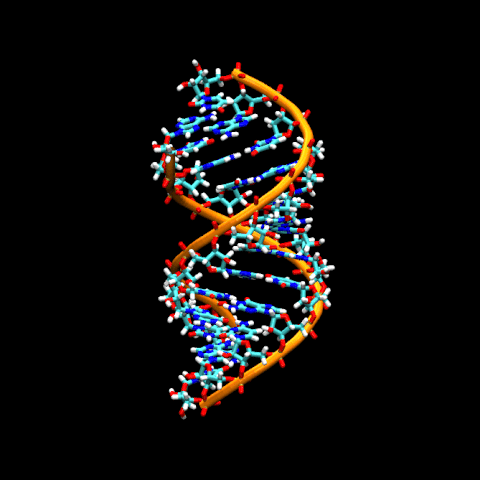
\includegraphics[width=\textwidth]{Plots/dsRNS.png}
	\end{minipage}
  \begin{minipage}{0.3\textwidth}
	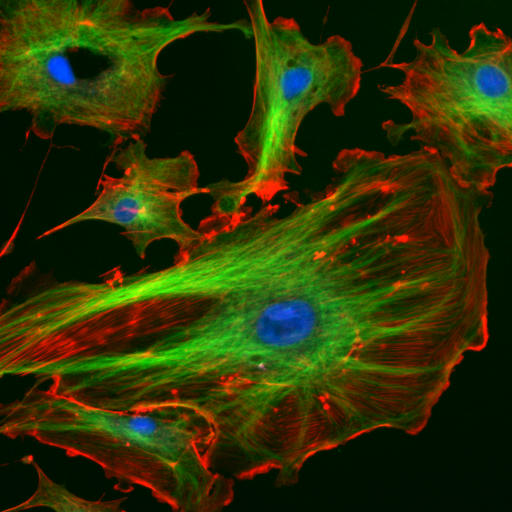
\includegraphics[width=\textwidth]{Plots/FluorescentCells.jpg}
	\end{minipage} \\
  \begin{minipage}{\textwidth}
    \begin{tiny}
       Quellen:\\
        links:  \url{https://en.wikipedia.org/wiki/RNA}\\%##/media/File:Double-stranded_RNA.gif} \\
        rechts: \url{https://de.wikipedia.org/wiki/Mikrotubulus}%##/media/File:FluorescentCells.jpg}\\
    \end{tiny}
  \end{minipage}

\end{frame}


%\begin{frame}{Embedded Animation}
%  \animategraphics[loop,controls,width=0.5\linewidth]{4}{Plots/dsRna/something-}{0}{94}
%\end{frame}
%
\begin{frame}
  \frametitle{Was ist ein neuronales Netz}
  \begin{minipage}{0.5\textwidth}
  \begin{itemize}
    \item Inspiriert durch das biologische Neuron-Modell
    \item Mensch besitzt ca. $10^{11}$ Neuronen in Großhirnrinde
  \end{itemize}
  \end{minipage}%
  \hfill%
  \begin{minipage}{0.5\textwidth}
    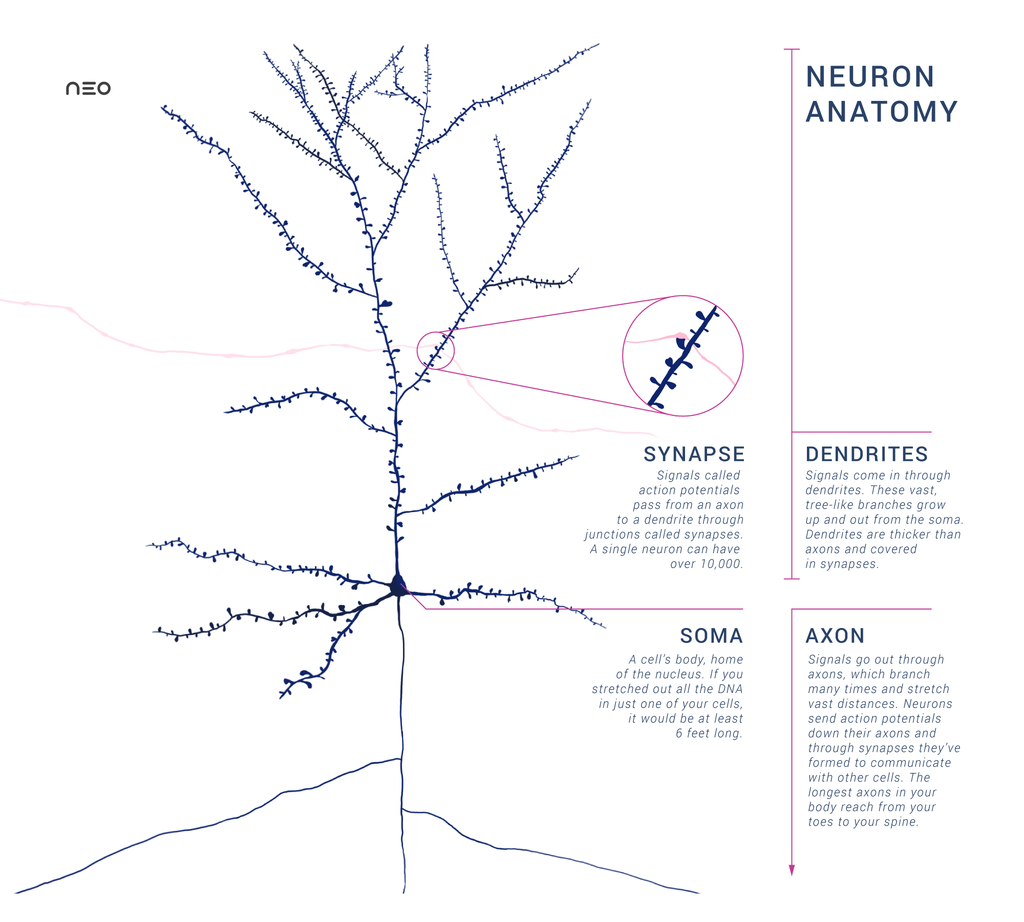
\includegraphics[width=\textwidth]{Plots/anatomy-neuron.png}
  \end{minipage}
  \begin{minipage}{\textwidth}
   \begin{tiny}
      Quelle: \\
      \url{https://en.wikipedia.org/wiki/Neuron}%##/media/File:Anatomy_of_a_Neuron_with_Synapse.png}
   \end{tiny}
  \end{minipage}
\end{frame}

\begin{frame}
\frametitle{Wieso Neuronale Netze?}
  \begin{itemize}
    \item Erfolgreicher Einsatz bei der Analyse von anderen Systemen\\
          \begin{itemize}
              \item 2d-Ising-Modell
              \item Hubbard-Modell
          \end{itemize}
    \item Ähnlichkeit zu Renormierungsgruppenmethoden (unsupervised learning)
    \item Generelle Idee:\\
        \begin{enumerate}
          \item Erzeugung von Trainingswerten mittels MC-Simulation
          \item Trainieren des Netzwerks mit den Trainingswerten
          \item Analyse von Messwerten
        \end{enumerate}
  \end{itemize}
\end{frame}
